% !TeX document-id = {c68f4be8-c497-43e0-82df-e9ebfbea9577}
% !TeX TXS-program:pdflatex = pdflatex -synctex=1 -interaction=nonstopmode --shell-escape %.tex
% новая команда \RNumb для вывода римских цифр
\documentclass[a4paper,12pt]{article}
\usepackage{amssymb}
\usepackage{amsmath}
\usepackage{amsthm}
\usepackage{caption}
\usepackage{misccorr}
\usepackage[noadjust]{cite}
\usepackage{cmap}
\usepackage[utf8x]{inputenc}
\usepackage[T2A]{fontenc}
\usepackage[english, russian]{babel}
\usepackage{graphics}
\usepackage{graphicx}
\usepackage{textcomp}
\usepackage{verbatim}
\usepackage{makeidx}
\usepackage{geometry}
\usepackage{float}
\usepackage{bm}
\usepackage{esint}
\usepackage{mathtools}
\usepackage{graphicx}
\usepackage{listings}
\usepackage{courier}
\usepackage{multirow}
\usepackage{graphicx}
\usepackage{xcolor}
\usepackage{ucs}
\usepackage{pdfpages}


\lstdefinestyle{asm}{
	language={[x86masm]Assembler},
	backgroundcolor=\color{white},
	basicstyle=\footnotesize\ttfamily,
	keywordstyle=\color{blue},
	stringstyle=\color{red},
	commentstyle=\color{gray},
	numbers=left,
	numberstyle=\tiny,
	stepnumber=1,
	numbersep=5pt,
	frame=single,
	tabsize=4,
	captionpos=b,
	breaklines=true
}

\lstset{basicstyle=\fontsize{10}{10}\selectfont,breaklines=true,inputencoding=utf8x,extendedchars=\true}

\lstset{
	literate=
	{а}{{\selectfont\char224}}1
	{б}{{\selectfont\char225}}1
	{в}{{\selectfont\char226}}1
	{г}{{\selectfont\char227}}1
	{д}{{\selectfont\char228}}1
	{е}{{\selectfont\char229}}1
	{ё}{{\"e}}1
	{ж}{{\selectfont\char230}}1
	{з}{{\selectfont\char231}}1
	{и}{{\selectfont\char232}}1
	{й}{{\selectfont\char233}}1
	{к}{{\selectfont\char234}}1
	{л}{{\selectfont\char235}}1
	{м}{{\selectfont\char236}}1
	{н}{{\selectfont\char237}}1
	{о}{{\selectfont\char238}}1
	{п}{{\selectfont\char239}}1
	{р}{{\selectfont\char240}}1
	{с}{{\selectfont\char241}}1
	{т}{{\selectfont\char242}}1
	{у}{{\selectfont\char243}}1
	{ф}{{\selectfont\char244}}1
	{х}{{\selectfont\char245}}1
	{ц}{{\selectfont\char246}}1
	{ч}{{\selectfont\char247}}1
	{ш}{{\selectfont\char248}}1
	{щ}{{\selectfont\char249}}1
	{ъ}{{\selectfont\char250}}1
	{ы}{{\selectfont\char251}}1
	{ь}{{\selectfont\char252}}1
	{э}{{\selectfont\char253}}1
	{ю}{{\selectfont\char254}}1
	{я}{{\selectfont\char255}}1
	{А}{{\selectfont\char192}}1
	{Б}{{\selectfont\char193}}1
	{В}{{\selectfont\char194}}1
	{Г}{{\selectfont\char195}}1
	{Д}{{\selectfont\char196}}1
	{Е}{{\selectfont\char197}}1
	{Ё}{{\"E}}1
	{Ж}{{\selectfont\char198}}1
	{З}{{\selectfont\char199}}1
	{И}{{\selectfont\char200}}1
	{Й}{{\selectfont\char201}}1
	{К}{{\selectfont\char202}}1
	{Л}{{\selectfont\char203}}1
	{М}{{\selectfont\char204}}1
	{Н}{{\selectfont\char205}}1
	{О}{{\selectfont\char206}}1
	{П}{{\selectfont\char207}}1
	{Р}{{\selectfont\char208}}1
	{С}{{\selectfont\char209}}1
	{Т}{{\selectfont\char210}}1
	{У}{{\selectfont\char211}}1
	{Ф}{{\selectfont\char212}}1
	{Х}{{\selectfont\char213}}1
	{Ц}{{\selectfont\char214}}1
	{Ч}{{\selectfont\char215}}1
	{Ш}{{\selectfont\char216}}1
	{Щ}{{\selectfont\char217}}1
	{Ъ}{{\selectfont\char218}}1
	{Ы}{{\selectfont\char219}}1
	{Ь}{{\selectfont\char220}}1
	{Э}{{\selectfont\char221}}1
	{Ю}{{\selectfont\char222}}1
	{Я}{{\selectfont\char223}}1
}

\newcommand{\specchapter}[1]{\chapter*{#1}\addcontentsline{toc}{chapter}{#1}}
\newcommand{\specsection}[1]{\section*{#1}\addcontentsline{toc}{section}{#1}}
\newcommand{\specsubsection}[1]{\subsection*{#1}\addcontentsline{toc}{subsection}{#1}}
\newcommand{\RNumb}[1]{\uppercase\expandafter{\romannumeral #1\relax}}
\newcommand{\jj}{\righthyphenmin=20 \justifying}


% геометрия
\geometry{pdftex, left = 2cm, right = 2cm, top = 2.5cm, bottom = 2.5cm}

\setcounter{tocdepth}{4} % фикс переноса 
\righthyphenmin = 2
\tolerance = 2048

\begin{document}
\thispagestyle{empty}

\noindent \begin{minipage}{0.15\textwidth}
	
\includegraphics[width=\linewidth]{logo}
\end{minipage}
\noindent\begin{minipage}{0.9\textwidth}\centering
	\textbf{Министерство науки и высшего образования Российской Федерации}\\
	\textbf{Федеральное государственное бюджетное образовательное учреждение высшего образования}\\
	\textbf{«Московский государственный технический университет имени Н.Э.~Баумана}\\
	\textbf{(национальный исследовательский университет)»}\\
	\textbf{(МГТУ им. Н.Э.~Баумана)}
\end{minipage}

\noindent\rule{18cm}{3pt}
\newline\newline
\noindent ФАКУЛЬТЕТ $\underline{\text{«Информатика и системы управления»}}$ \newline\newline
\noindent КАФЕДРА $\underline{\text{«Программное обеспечение ЭВМ и информационные технологии»}}$\newline\newline\newline\newline\newline\newline\newline


\begin{center}
	\noindent\begin{minipage}{1.3\textwidth}\centering
	\Large\textbf{   ~~~ Лабораторная работа №1 (часть 1)}\newline
	\textbf{по дисциплине "Операционные системы"}\newline\newline\newline
	\end{minipage}
\end{center}

\noindent\textbf{Тема} $\underline{\text{Дизассемблирование INT 8h}}$\newline\newline
\noindent\textbf{Студент} $\underline{\text{Савинова М. Г.}}$\newline\newline
\noindent\textbf{Группа} $\underline{\text{ИУ7-51Б}}$\newline\newline
\noindent\textbf{Преподаватель} $\underline{\text{Рязанова Н. Ю.}}$\newline

\begin{center}
	\vfill
	Москва~---~\the\year
~г.
\end{center}
\clearpage

\section{Полученный дизассемблированный код}

\subsection{Листинг обработчика прерывания INT 8h} 
\begin{lstlisting}[style={asm}]
;; Вызов процедуры sub_7 (запрет прерываний)
020A:0746  E8 0070				call	sub_7			; (07B9)

;; Сохраненние содержимого регистров ES, DS, AX, DX
020A:0749  06					push	es
020A:074A  1E					push	ds
020A:074B  50					push	ax
020A:074C  52					push	dx

;; В регистр DS загружается адрес 0040:0000
; начало области данных BIOS (через буфер AX)
020A:074D  B8 0040				mov	ax,40h
020A:0750  8E D8				mov	ds,ax

;; В регистр ES загружается адрес 0000:0000
; адрес начала таблицы векторов прерываний (через буфер AX)
020A:0752  33 C0				xor	ax,ax			; Zero register
020A:0754  8E C0				mov	es,ax

;; инкремент счетчика таймера
;; инкремент младшей части счетчика таймера
020A:0756  FF 06 006C				inc	word ptr ds:[6Ch]	; (0040:006C=0A098h)

;; если младшая часть счетчика CB == 0, 
; то инкремент двух старших байтов CB
; иначе переходим на loc_19
020A:075A  75 04				jnz	loc_19			; Jump if not zero

;; снкремент старшей части счетчика CB
020A:075C  FF 06 006E				inc	word ptr ds:[6Eh]	; (0040:006E=0)

;; сброс счетчика CB и выставление флага окончания суток

;; если два старших байта счетчика CB == 24
; то сравниваем два младших байта счетчика CB,
; иначе декремент счетчика CB до отключения моторчика дисковода
020A:0760			loc_19:
020A:0760  83 3E 006E 18			cmp	word ptr ds:[6Eh],18h	; (0040:006E=0)
020A:0765  75 15				jne	loc_20			; Jump if not equal

;; если два старших байта счетчика CB == 176
; то обнуление счетчика CB и установка флага прошедших суток
; иначе декремент счетчика CB до отключения моторчика дисковода
020A:0767  81 3E 006C 00B0			cmp	word ptr ds:[6Ch],0B0h	; (0040:006C=0A098h)

;; обнуляем счетчик ( если прошел день )
020A:076D  75 0D				jne	loc_20			; Jump if not equal
020A:076F  A3 006E				mov	word ptr ds:[6Eh],ax	
; (0040:006E=0) обнуляем счетчик (старшая часть)

020A:0772  A3 006C				mov	word ptr ds:[6Ch],ax	
; (0040:006C=0A098h) (младшая часть)

;; в ячейку 0040::0070 записываем единицу
; для фиксации о том, что новый день наступил

020A:0775  C6 06 0070 01			mov	byte ptr ds:[70h],1	; (0040:0070=0)
020A:077A  0C 08				or	al,8

;; декремент счетчика до отключения моторчика дисковода
020A:077C			loc_20:
020A:077C  50					push	ax
020A:077D  FE 0E 0040				dec	byte ptr ds:[40h]	; (0040:0040=63h)

;; если значение этого счетчика == 0
; то установка флага отключения моторчика и посылка команды в порт на отключение моторчика
020A:0781  75 0B				jnz	loc_21			; Jump if not zero
020A:0783  80 26 003F F0			and	byte ptr ds:[3Fh],0F0h	; (0040:003F=0)
020A:0788  B0 0C				mov	al,0Ch
020A:078A  BA 03F2				mov	dx,3F2h
020A:078D  EE					out	dx,al			; port 3F2h, dsk0 contrl output

;; проверка, установлен ли PF, т. е. разрешен ли ответ на маскиреумые прерывания
020A:078E			loc_21:
020A:078E  58					pop	ax

;; проверка флага PF по адресу 0040:0314
; (0100, поднят 2 бит, отвечает за флаг PF, флаг четности)
020A:078F  F7 06 0314 0004			test	word ptr ds:[314h],4	; (0040:0314=3200h)

;; если вызов маскируемых прерываний разрешен, переход к вызову int 1Ch (в loc_22)
020A:0795  75 0C				jnz	loc_22			; Jump if not zero
020A:0797  9F					lahf				; Load ah from flags
020A:0798  86 E0				xchg	ah,al
020A:079A  50					push	ax

;; иначе, косвенный вызов 1Ch - как процедуры командой call и переход к loc_23
; ( 1C * 4 = 70h )
020A:079B  26: FF 1E 0070			call	dword ptr es:[70h]	; (0000:0070=6ADh)
020A:07A0  EB 03				jmp	short loc_23		; (07A5)
020A:07A2  90					nop

;; вызов пользовательского прерывания по таймеру
020A:07A3			loc_22:
020A:07A3  CD 1C				int	1Ch			; Timer break (call each 18.2ms)
;; после инициализации системы вектор INt 1Ch указывает на команду IRET 

; сброс конроллера прерываний
020A:07A5			loc_23:
020A:07A5  E8 0011				call	sub_7			; (07B9)
020A:07A8  B0 20				mov	al,20h			; ' '
020A:07AA  E6 20				out	20h,al			; port 20h, 8259-1 int command
										;  al = 20h, end of interrupt
;; восстановление значений регистров
020A:07AC  5A					pop	dx
020A:07AD  58					pop	ax
020A:07AE  1F					pop	ds
020A:07AF  07					pop	es

;;прыжок в адрес 020А:064С
020A:07B0  E9 FE99				jmp	loc_3			; (064C)

;...

020A:064C			loc_3:
020A:064C  1E					push	ds
020A:064D  50					push	ax

;...

020A:06AA  58					pop	ax
020A:06AB  1F					pop	ds
020A:06AC  CF					iret				; Interrupt return
\end{lstlisting}

% \clearpage
\subsection{Листинг процедуры sub\_7}

\begin{lstlisting}[style={asm}]
				sub_7		proc	near
;; Соохранение содержимого регистров DS, AX
020A:07B9  1E					push	ds
020A:07BA  50					push	ax

;; В регистр DS загружается адрес 0040:0000 начало области данных BIOS
020A:07BB  B8 0040				mov	ax,40h
020A:07BE  8E D8				mov	ds,ax

;; Загрузка младшего байта регистра EFLAGS в A
020A:07C0  9F					lahf				; Load ah from flags

;; Если флаг DF == 0 и старший бит IOLP == 0
; то сброс флага разрешения прерывания IF в 0040:0314
; иначе запрет маскируемых прерываний инструкцией CLI
020A:07C1  F7 06 0314 2400			test	word ptr ds:[314h],2400h	; (0040:0314=3200h)
020A:07C7  75 0C				jnz	loc_25			; Jump if not zero

;; Сброс флага IF
020A:07C9  F0> 81 26 0314 FDFF	           lock	and	word ptr ds:[314h],0FDFFh	; (0040:0314=3200h)

;; Восстановление значений флагов
020A:07D0			loc_24:
020A:07D0  9E					sahf				; Store ah into flags

;; Восстановление значений регистров
020A:07D1  58					pop	ax
020A:07D2  1F					pop	ds
020A:07D3  EB 03				jmp	short loc_26		; (07D8)

;; Сброс IF, т. е. запрет прерываний с помощью команды cli
020A:07D5			loc_25:
020A:07D5  FA					cli				; Disable interrupts
020A:07D6  EB F8				jmp	short loc_24		; (07D0)

;; Выход из программы
020A:07D8			loc_26:
020A:07D8  C3					retn
				sub_7		endp
\end{lstlisting}
\clearpage

\section{Схема алгоритмов}

\subsection{Схема алгоритма обработчика INT8h}
% ""\newline

\begin{center}
    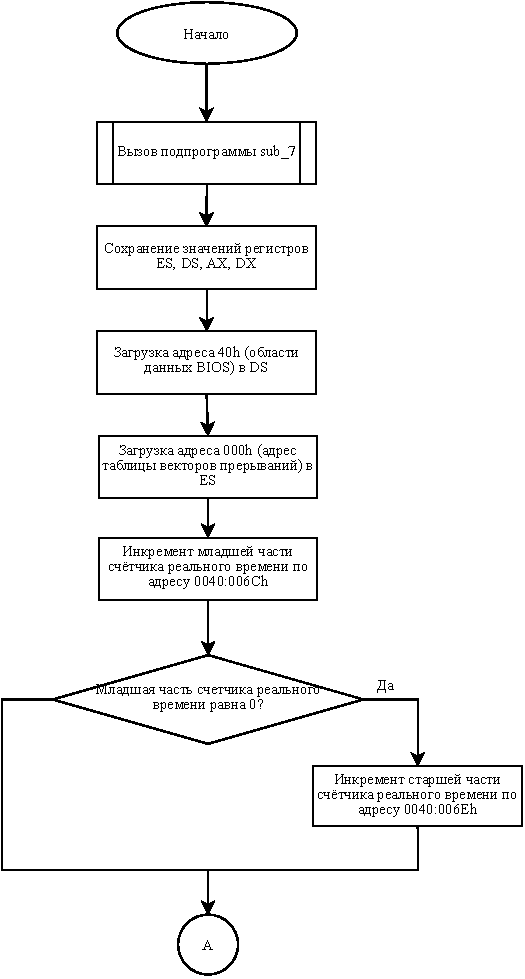
\includegraphics[height=0.9\textheight]{flowchart/1.pdf}
    \newpage
    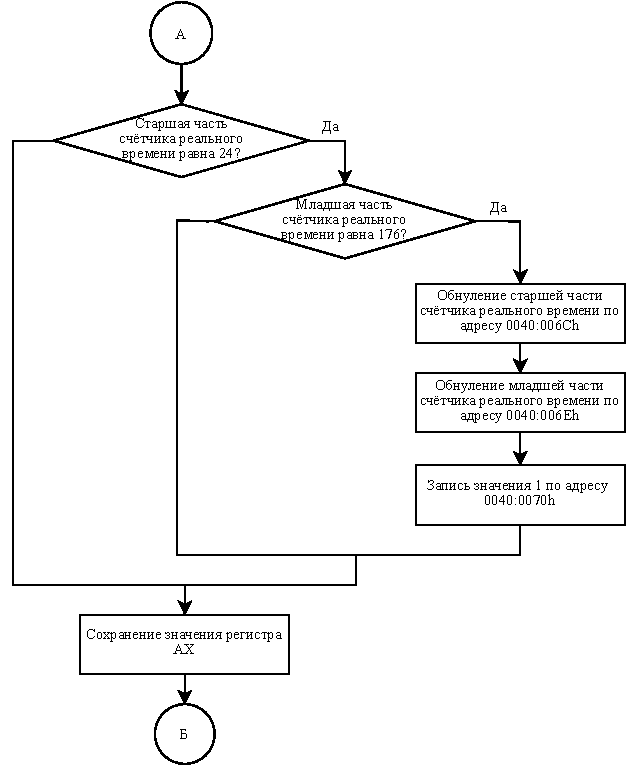
\includegraphics[height=0.9\textheight]{flowchart/2.pdf}
    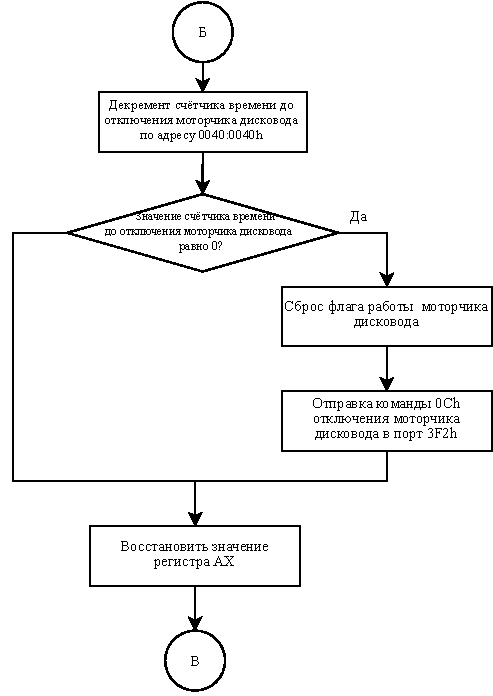
\includegraphics[height=0.95\textheight]{flowchart/3.pdf}
    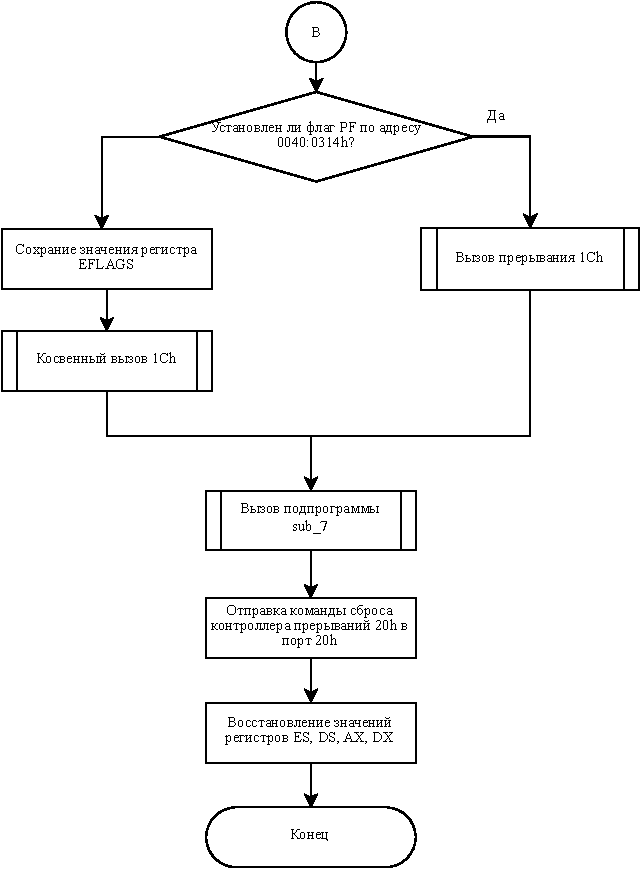
\includegraphics[height=0.95\textheight]{flowchart/4.pdf}
\end{center}

% \clearpage
\subsection{Схема алгоритма процедуры sub\_7}
    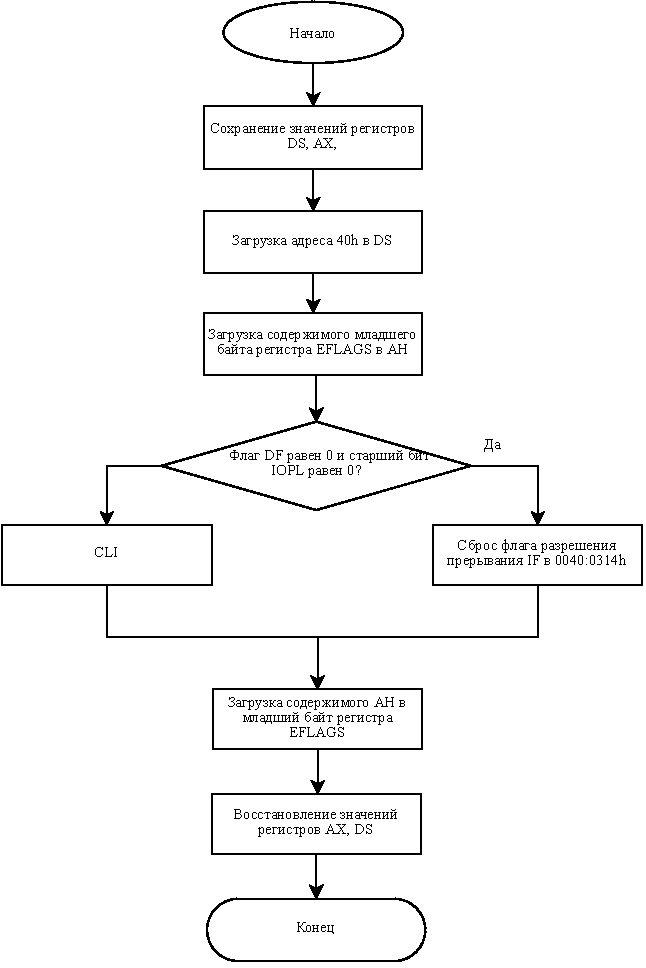
\includegraphics[height=0.95\textheight]{flowchart/5.pdf}
\begin{center}
\end{center}

\end{document}